\chapter{Asynchroniczny przerzutnik R-S}

\begin{itemize}
    \item Schemat razem z rozpiską pinów:
        \begin{figure}[H]
            \centering
            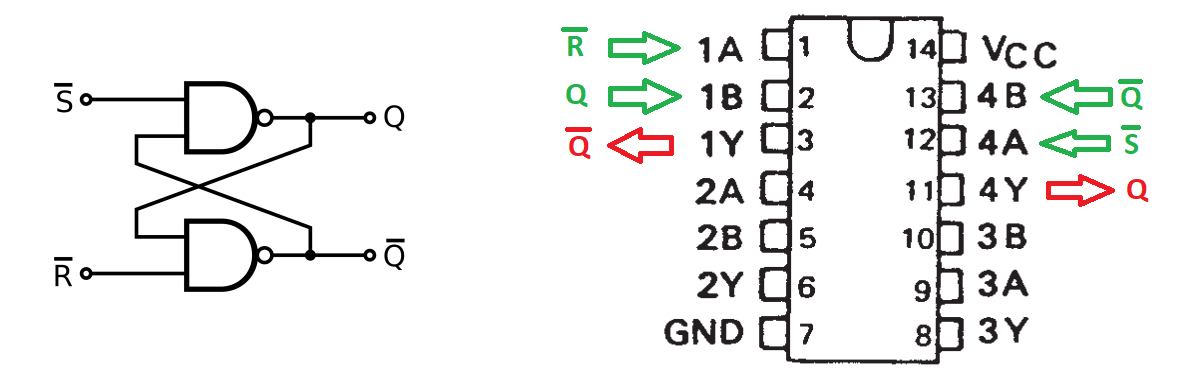
\includegraphics[width=\textwidth]{img/schemes_with_pins/przerzutnik_w_pins.png}
            \label{przerzutnik:schemat_w_pins}
        \end{figure}
    \item Zbudowany przerzutnik:
        \begin{figure}[H]
            \centering
            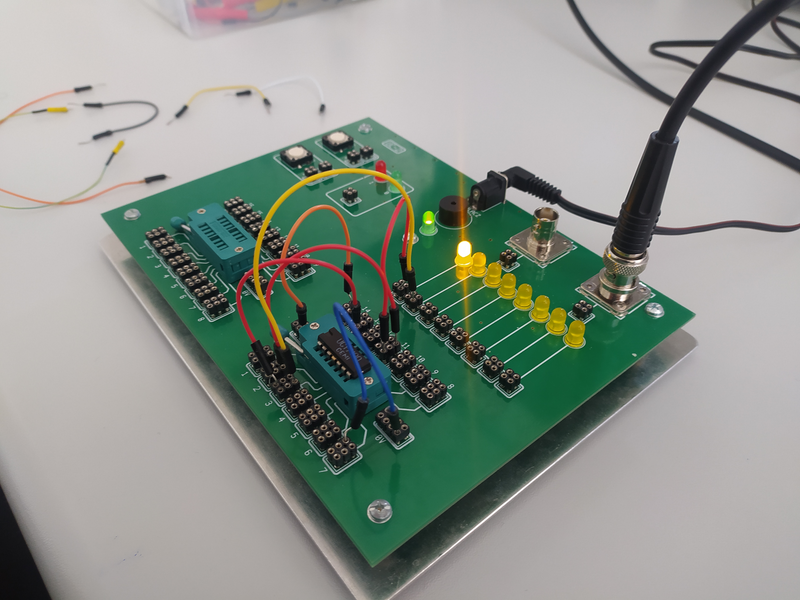
\includegraphics[width=\textwidth]{img/przerzutnik/1652306732322_scaled.png}
            \caption{Zbudowany przerzutnik}
            \label{przerzutnik:zbudowany}
        \end{figure}
        
\pagebreak

    \item Po odłączeniu sygnałów wejściowych przerzutnik pamięta ostatnio zapisany stan:
        \begin{figure}[H]
            \centering
            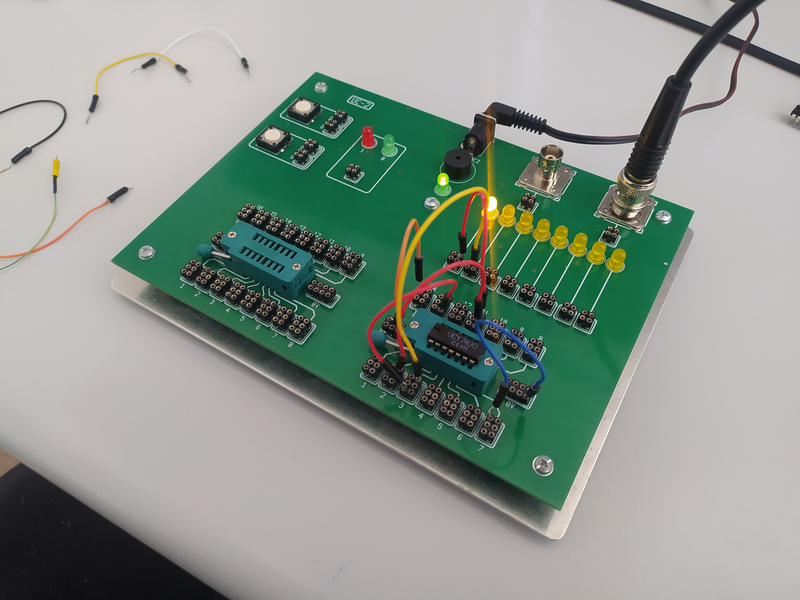
\includegraphics[width=\textwidth]{img/przerzutnik/1652306732331_scaled.png}
            \caption{Zapamiętany stan}
            \label{przerzutnik:pamietanie}
        \end{figure}
        
    \item Przerzutnik zachowuje się zgodnie z przewidywaniami.
\end{itemize}